\chapter{Theoretical Foundations}
\label{ch:theory}

This chapter establishes the theoretical foundation for the central problem of this thesis: predicting multi-crystal sedimentation flows using machine learning. We first review the physics of crystal settling in the creeping-flow regime and motivate the stream-function formulation adopted in this work (\S\ref{sec:crystal_physics}). We then introduce U-Net architectures for structured flow-field prediction (\S\ref{sec:unet}), discuss physics-informed learning strategies and their relation to the present approach (\S\ref{sec:pinns}), and finally analyze the generalization problem of training on $N$-crystal configurations while evaluating on $1$ to $N$ crystals (\S\ref{sec:generalization}).

% ----------------------------------------------------------------------------
\section{Physics of Crystal Sedimentation}
\label{sec:crystal_physics}
% ----------------------------------------------------------------------------

\subsection{Stokes Flow Fundamentals}

Crystal sedimentation in magmatic environments typically occurs at very low Reynolds numbers, where viscous forces dominate over inertia. The dynamics of the carrier fluid are then governed by the Stokes equations
\begin{align}
\mathbf{0} &= -\nabla p + \mu \nabla^2 \mathbf{u} + \rho \mathbf{g}, 
\label{eq:stokes_momentum}\\[0.2em]
\nabla \cdot \mathbf{u} &= 0,
\label{eq:stokes_incompressible}
\end{align}
where $\mathbf{u}$ is the fluid velocity, $p$ is pressure, $\mu$ is dynamic viscosity, $\rho$ is density, and $\mathbf{g}$ is gravitational acceleration. The incompressibility condition~\eqref{eq:stokes_incompressible} ensures volume conservation.

The creeping-flow regime is characterized by a small Reynolds number
\begin{equation}
\mathrm{Re} = \frac{\rho_f \, U \, D}{\mu} \ll 1,
\end{equation}
where $U$ and $D$ are typical velocity and length scales of the problem and $\rho_f$ is the fluid density. Under these conditions, the flow field adjusts quasi-instantaneously to changes in geometry, and time dependence is often neglected when considering steady sedimentation.

For a single isolated spherical particle of diameter $D$ and density $\rho_p$ settling in a quiescent Newtonian fluid of viscosity $\mu$ and density $\rho_f$, classical solutions \parencite{stokes_mathematical_2009,happel_low_1991} give the terminal settling velocity
\begin{equation}
v_s = \frac{1}{18} \frac{\left(\rho_p - \rho_f\right) g}{\mu} D^2,
\label{eq:stokes_law}
\end{equation}
which provides a baseline estimate for crystal descent in magmatic chambers \parencite{martin_crystal_1988}. Equation~\eqref{eq:stokes_law} highlights the strong sensitivity of $v_s$ to crystal size and viscosity, two key parameters in petrological applications.

\subsection{Stream-Function Formulation}

For two-dimensional incompressible flow in the $(x,z)$-plane, it is convenient to introduce a stream function $\psi(x,z)$ such that
\begin{equation}
\mathbf{u}(x,z) = 
\begin{pmatrix}
u_x \\[0.2em] u_z
\end{pmatrix}
=
\begin{pmatrix}
\;\;\dfrac{\partial \psi}{\partial z} \\[0.6em]
-\dfrac{\partial \psi}{\partial x}
\end{pmatrix}
= \nabla \times \left(\psi \,\mathbf{e}_y\right),
\label{eq:streamfunction_def}
\end{equation}
where $\mathbf{e}_y$ is the unit vector normal to the $(x,z)$-plane. By construction, definition~\eqref{eq:streamfunction_def} satisfies incompressibility exactly, since
\begin{equation}
\nabla \cdot \mathbf{u} = 
\frac{\partial u_x}{\partial x} + \frac{\partial u_z}{\partial z}
= \frac{\partial^2 \psi}{\partial x \partial z}
- \frac{\partial^2 \psi}{\partial z \partial x} = 0.
\end{equation}

Contours of constant $\psi$ correspond to streamlines of the flow, and changes in $\psi$ across a band are proportional to volumetric flux. Figure~\ref{fig:streamfunction_schematic} schematically illustrates a stream-function representation around a rigid circular inclusion. The blue lines indicate constant-$\psi$ curves, which wrap around the crystal and encode the local deflection of the flow. Because $\mathbf{u}$ can be reconstructed uniquely (up to an additive constant in $\psi$) via~\eqref{eq:streamfunction_def}, learning $\psi$ is an attractive target for surrogate modeling: a sufficiently accurate approximation of $\psi$ yields a divergence-free velocity field by construction.

\begin{figure}[ht]
\centering
% (TikZ code as provided; geometry may be adjusted later)
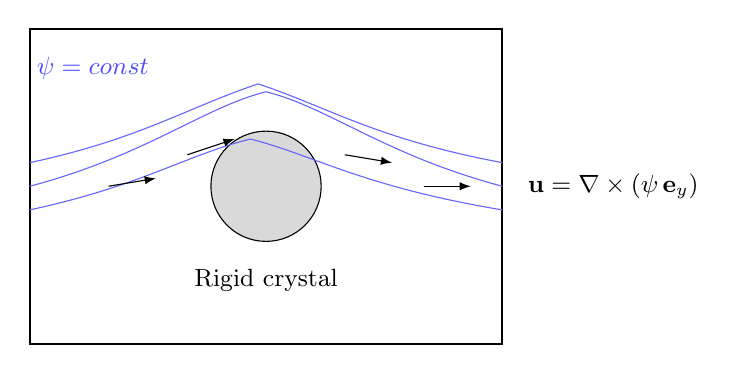
\begin{tikzpicture}[font=\small,>=latex,scale=1.0]

% Domain
\draw[thick] (-3,-2) rectangle (3,2);

% Circular inclusion
\draw[fill=gray!30] (0,0) circle (0.7);

% Streamlines (schematic)
\draw[blue!60] (-3,0.0) .. controls (-1.5,0.4) and (-0.8,1.0) .. (0,1.2)
               .. controls (0.8,1.0) and (1.5,0.4) .. (3,0.0);
\draw[blue!60] (-3,-0.3) .. controls (-1.6,0.0) and (-1.0,0.4) .. (-0.2,0.6)
               .. controls (0.6,0.4) and (1.2,0.0) .. (3,-0.3);
\draw[blue!60] (-3,0.3) .. controls (-1.6,0.6) and (-1.0,1.0) .. (-0.1,1.3)
               .. controls (0.8,1.0) and (1.4,0.6) .. (3,0.3);

% Velocity arrows (schematic)
\draw[->] (-2,0) -- (-1.4,0.1);
\draw[->] (-1,0.4) -- (-0.4,0.6);
\draw[->] (1,0.4) -- (1.6,0.3);
\draw[->] (2,0.0) -- (2.6,0.0);

% Labels
\node[blue!70] at (-2.2,1.5) {$\psi = \text{const}$};
\node at (0,-1.2) {Rigid crystal};
\node[anchor=west] at (3.2,0.0) {$\mathbf{u} = \nabla \times (\psi\,\mathbf{e}_y)$};

\end{tikzpicture}
\caption{Schematic representation of a stream-function formulation around a rigid inclusion. Contours $\psi = \text{const}$ correspond to streamlines of an incompressible flow field. Given $\psi$, the velocity field can be reconstructed via equation~\eqref{eq:streamfunction_def}.}
\label{fig:streamfunction_schematic}
\end{figure}

The vorticity $\omega$ associated with the velocity field is defined by
\begin{equation}
\omega = (\nabla \times \mathbf{u})_y
= \frac{\partial u_z}{\partial x} - \frac{\partial u_x}{\partial z}.
\end{equation}
In the stream-function formulation, $\omega$ and $\psi$ are linked by the Poisson equation
\begin{equation}
\Delta \psi = - \omega,
\label{eq:poisson_psi}
\end{equation}
subject to appropriate boundary conditions. This relationship is central for the data generation and normalization procedures used later in this thesis.

\subsection{From Stokes Equations to Poisson and Biharmonic Equations}
\label{sec:psi_poisson_derivation}

For completeness, we briefly derive the Poisson equation~\eqref{eq:poisson_psi} and the associated biharmonic equation for $\psi$ starting from the incompressible Stokes equations. The derivation also clarifies how different notational variants, $\Delta \psi$ versus $\nabla^2 \psi$ and $\Delta^2 \psi$, arise.

\paragraph{Kinematic relation between vorticity and stream function.}
\\
Using the stream-function representation~\eqref{eq:streamfunction_def}, the $y$-component of vorticity is
\begin{align}
\omega 
&= (\nabla \times \mathbf{u})_y
 = \frac{\partial u_z}{\partial x} - \frac{\partial u_x}{\partial z} \\[0.2em]
&= \frac{\partial}{\partial x}\!\left(-\frac{\partial \psi}{\partial x}\right)
   - \frac{\partial}{\partial z}\!\left(\frac{\partial \psi}{\partial z}\right) \\[0.2em]
&= -\frac{\partial^2 \psi}{\partial x^2}
   -\frac{\partial^2 \psi}{\partial z^2}
 = -\Delta \psi.
\end{align}
Thus we immediately recover the Poisson equation
\begin{equation}
\Delta \psi = -\omega.
\end{equation}
This relation is purely kinematic: it contains no information about viscosity, pressure, or body forces, and holds for any sufficiently smooth, incompressible two-dimensional flow. The notation $\nabla^2 \psi$ is completely equivalent to $\Delta \psi$ and simply emphasizes that $\Delta$ is the Laplace operator.

\paragraph{Dynamic relation and the biharmonic equation.}

To obtain an equation involving $\psi$ alone, we return to the Stokes momentum balance~\eqref{eq:stokes_momentum}. For constant viscosity and in the absence of rotational body forces, the gravitational term can be absorbed into the pressure, and we may write
\begin{equation}
\mathbf{0} = -\nabla p + \mu \nabla^2 \mathbf{u}.
\end{equation}
Taking the curl of this equation eliminates the pressure, since $\nabla \times \nabla p = \mathbf{0}$, and yields
\begin{equation}
\mathbf{0} = \nabla \times (\mu \nabla^2 \mathbf{u})
          = \mu\, \nabla \times (\nabla^2 \mathbf{u}).
\end{equation}
For sufficiently smooth fields, the Laplacian and curl commute, so that
\begin{equation}
\nabla \times (\nabla^2 \mathbf{u})
= \nabla^2 (\nabla \times \mathbf{u})
= \nabla^2 \boldsymbol{\omega}.
\end{equation}
Consequently, the vorticity satisfies
\begin{equation}
\nabla^2 \boldsymbol{\omega} = \mathbf{0},
\end{equation}
which, in our two-dimensional setting with only a $y$-component of vorticity, reduces to
\begin{equation}
\Delta \omega = 0.
\label{eq:laplace_omega}
\end{equation}
Combining~\eqref{eq:laplace_omega} with the kinematic relation $\omega = -\Delta \psi$ yields
\begin{equation}
\Delta(-\Delta \psi) = 0
\quad\Rightarrow\quad
\Delta^2 \psi = 0,
\label{eq:biharmonic_psi}
\end{equation}
the classical \emph{biharmonic equation} for the stream function in steady Stokes flow with constant viscosity and no rotational body forces.

From a numerical perspective, equations~\eqref{eq:poisson_psi} and~\eqref{eq:biharmonic_psi} serve different purposes. The Poisson equation $\Delta \psi = -\omega$ is a second-order elliptic problem that is comparatively easy to discretize and solve with standard finite-difference or finite-element methods. In this thesis, the vorticity $\omega$ and velocity field $\mathbf{u}$ are obtained from LaMEM, which already solves the full Stokes system. The Poisson equation is then solved on the resulting grid to construct a consistent stream function $\psi$.

In contrast, solving the biharmonic equation $\Delta^2 \psi = 0$ directly would require discretizing a fourth-order operator. This leads to wider finite-difference stencils, more involved finite-element formulations, and more delicate boundary conditions, all of which increase implementation complexity. Since LaMEM already provides high-quality Stokes solutions, it is more efficient and robust in the present context to compute $\psi$ via the Poisson problem with $\omega$ taken from LaMEM rather than solving the biharmonic equation as a stand-alone PDE.

\subsection{Multi-Crystal Interactions and Collective Behaviour}

When multiple crystals are present, hydrodynamic interactions lead to rich collective dynamics that cannot be inferred from single-particle behaviour alone. Even in the simplest case of two particles settling in tandem, wake interactions give rise to the canonical drafting–kissing–tumbling (DKT) sequence \parencite{fortes_nonlinear_1987}. As illustrated schematically in Figure~\ref{fig:dkt_sequence}, a trailing particle initially accelerates in the low-pressure wake of the leading particle (drafting), then approaches and briefly forms a near-contact pair (kissing), before the pair undergoes lateral separation and reorientation (tumbling).

\begin{figure}[ht]
\centering
% (TikZ code as provided; sizes can be tuned later)
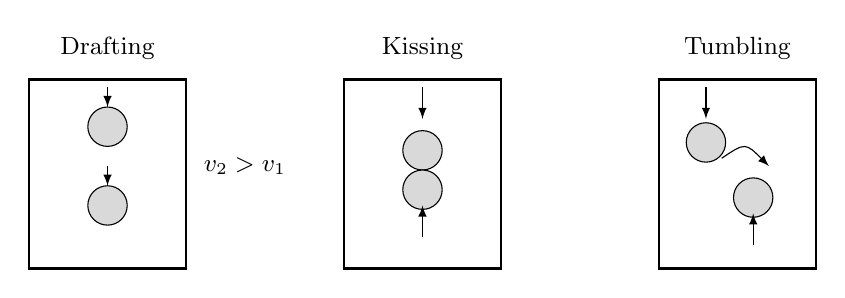
\begin{tikzpicture}[font=\small,>=latex]

% Panel 1: Drafting
\node at (0,2.8) {Drafting};
\draw[thick] (-1,0) rectangle (1,2.4);
\draw[fill=gray!30] (0,1.8) circle (0.25); % leading particle
\draw[fill=gray!30] (0,0.8) circle (0.25); % trailing particle
\draw[->] (0,2.3) -- (0,2.05);
\draw[->] (0,1.3) -- (0,1.05);
\node[anchor=west] at (1.1,1.3) {$v_2 > v_1$};

% Panel 2: Kissing
\node at (4,2.8) {Kissing};
\draw[thick] (3,0) rectangle (5,2.4);
\draw[fill=gray!30] (4,1.5) circle (0.25);
\draw[fill=gray!30] (4,1.0) circle (0.25);
\draw[->] (4,2.3) -- (4,1.9);
\draw[->] (4,0.4) -- (4,0.8);

% Panel 3: Tumbling
\node at (8,2.8) {Tumbling};
\draw[thick] (7,0) rectangle (9,2.4);
\draw[fill=gray!30] (7.6,1.6) circle (0.25);
\draw[fill=gray!30] (8.2,0.9) circle (0.25);
\draw[->] (7.6,2.3) -- (7.6,1.9);
\draw[->] (8.2,0.3) -- (8.2,0.7);
\draw[->] (7.8,1.4) .. controls (8.1,1.6) .. (8.4,1.3);

\end{tikzpicture}
\caption{Canonical drafting–kissing–tumbling (DKT) sequence for two settling particles. Hydrodynamic wake interactions first accelerate the trailing particle (drafting), then bring particles into near-contact (kissing), followed by lateral reorganization and separation (tumbling).}
\label{fig:dkt_sequence}
\end{figure}

At higher solid fractions, many-body interactions lead to hindered or enhanced settling, particle clustering, and large-scale pattern formation. Hindered settling is frequently described by the Richardson–Zaki relation
\begin{equation}
\frac{v}{v_0} = (1 - \phi)^n,
\label{eq:richardson_zaki}
\end{equation}
where $v$ is the effective settling velocity at particle volume fraction $\phi$, $v_0$ is the single-particle velocity, and $n$ is an empirical exponent depending on the Reynolds number and particle shape. Experiments and simulations in particle-laden geophysical flows \parencite{uhlmann_sedimentation_2014,penlou_experimental_2023,nissanka_dynamics_2023} show that wake-induced clustering, near-field lubrication forces, and long-range hydrodynamic coupling jointly control the macroscopic evolution of crystal populations.

\subsection{Scaling with Crystal Number}

The computational and physical complexity of multi-crystal sedimentation grows rapidly with the number of crystals $N$. A configuration with $N$ particles in two dimensions can be parameterized by $2N$ position coordinates and, in general, $N$ radii or shape parameters. Additionally, the number of distinct particle pairs scales as $N(N-1)/2$, leading to an effective $\mathcal{O}(N^2)$ growth in pairwise hydrodynamic interactions. High-fidelity numerical solvers must resolve both the boundary layers around each particle and the long-range disturbance fields, resulting in large linear systems with poor conditioning \parencite{glowinski_fictitious_2001}.

Figure~\ref{fig:n_scaling} illustrates this conceptual scaling by plotting a schematic $\mathcal{O}(N^2)$ curve for the relative computational cost as a function of $N$. Although the precise scaling depends on the numerical method and implementation, fully resolved simulations for $N \gtrsim 10$ become increasingly expensive, motivating the use of surrogate models that approximate the mapping from crystal configurations to flow fields.

\begin{figure}[ht]
\centering
% (pgfplots code; the precise curve and axis limits can be tuned later)
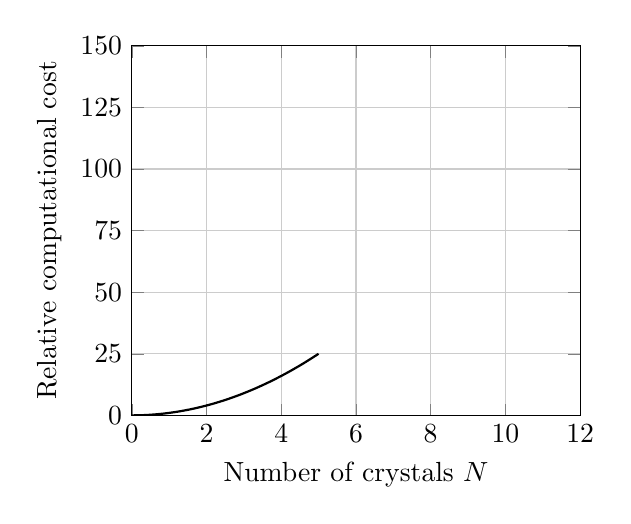
\begin{tikzpicture}
\begin{axis}[
    width=0.6\textwidth,
    xlabel={Number of crystals $N$},
    ylabel={Relative computational cost},
    xmin=0, xmax=12,
    ymin=0, ymax=150,
    xtick={0,2,4,6,8,10,12},
    ytick={0,25,50,75,100,125,150},
    grid=both,
    minor grid style={gray!20},
    major grid style={gray!40},
]
\addplot[smooth,thick] {x^2};
\end{axis}
\end{tikzpicture}
\caption{Conceptual scaling of computational complexity with the number of crystals $N$. Fully resolved methods exhibit effectively quadratic growth due to pairwise hydrodynamic interactions, motivating surrogate approaches for $N \gtrsim 10$.}
\label{fig:n_scaling}
\end{figure}

% ----------------------------------------------------------------------------
\section{U-Net Architectures for Flow-Field Prediction}
\label{sec:unet}
% ----------------------------------------------------------------------------

\subsection{Encoder–Decoder Structure and Skip Connections}

U-Nets \parencite{navab_u-net_2015} are fully convolutional encoder–decoder architectures originally developed for biomedical image segmentation. Their structure is particularly well suited for learning mappings between structured inputs and outputs defined on the same grid, such as the mapping from crystal geometries to flow fields.

A typical U-Net consists of:
\begin{itemize}
    \item a \textbf{contracting path}, where convolutional blocks and downsampling layers extract progressively coarser-scale features;
    \item an \textbf{expanding path}, where upsampling and convolutional layers reconstruct a high-resolution output field;
    \item \textbf{skip connections}, where feature maps from the contracting path are concatenated with corresponding layers in the expanding path to preserve high-frequency information.
\end{itemize}

In the context of this thesis, the input to the U-Net is a multi-channel representation of the crystal configuration and auxiliary fields on a $256\times256$ grid (e.g., phase mask, signed distance function, and normalized coordinates), while the output is either a normalized stream-function field $\psi_{\text{norm}}$ or a residual field. The encoder captures global patterns such as large-scale recirculation or wake structures, whereas the decoder reconstructs smooth, high-resolution fields with sharp features near crystal boundaries.

Figure~\ref{fig:unet_architecture} shows a schematic U-Net architecture adapted for this problem. Boxes represent convolutional blocks, and arrows indicate the flow of information through the network. Skip connections link encoder and decoder stages at the same effective resolution, which is crucial for resolving narrow boundary layers and localized flow features around the crystals.

\begin{figure}[ht]
\centering
% (TikZ code; layout and sizes can be refined later)
\begin{tikzpicture}[font=\small,>=latex,node distance=1.8cm]

\tikzstyle{block}=[draw,minimum width=2.6cm,minimum height=1.1cm,align=center,rounded corners]

% Input
\node[block,fill=blue!10] (input) {Input\\Crystal Mask (+ Features)};

% Encoder
\node[block,fill=blue!20,right=of input] (enc1) {Conv Block 1};
\node[block,fill=blue!30,right=of enc1] (enc2) {Conv Block 2};
\node[block,fill=blue!40,right=of enc2] (enc3) {Conv Block 3};

% Bottleneck
\node[block,fill=orange!40,right=of enc3] (bottleneck) {Bottleneck};

% Decoder
\node[block,fill=green!40,above right=0.8cm and 1.5cm of bottleneck] (dec3) {Up + Conv};
\node[block,fill=green!30,above left=0.8cm and 1.5cm of dec3] (dec2) {Up + Conv};
\node[block,fill=green!20,above left=0.8cm and 1.5cm of dec2] (dec1) {Up + Conv};

% Output
\node[block,fill=red!20,left=2.3cm of dec1] (output) {Output\\$\psi_{\text{norm}}$ or Residual};

% Arrows encoder
\draw[->] (input) -- (enc1);
\draw[->] (enc1) -- (enc2);
\draw[->] (enc2) -- (enc3);
\draw[->] (enc3) -- (bottleneck);

% Arrows decoder
\draw[->] (bottleneck) -- (dec3);
\draw[->] (dec3) -- (dec2);
\draw[->] (dec2) -- (dec1);
\draw[->] (dec1) -- (output);

% Skip connections
\draw[->,thick] (enc3.north) -- ++(0,0.7) -| (dec3.west);
\draw[->,thick] (enc2.north) -- ++(0,0.9) -| (dec2.west);
\draw[->,thick] (enc1.north) -- ++(0,1.1) -| (dec1.west);

\end{tikzpicture}
\caption{Schematic U-Net architecture used for flow-field prediction. A convolutional encoder–decoder with skip connections maps crystal geometries and auxiliary features to stream-function or residual fields on a $256\times256$ grid.}
\label{fig:unet_architecture}
\end{figure}

\subsection{Loss Design and Normalization}

Given a training sample with input tensor $\mathbf{x}$ and target stream-function field $\psi$, the network predicts a normalized field $\hat{\psi}_{\text{norm}}(\mathbf{x})$. The corresponding loss function is typically chosen as a pixel-wise mean squared error
\begin{equation}
\mathcal{L}_\mathrm{data} 
= \frac{1}{N_\mathrm{pix}} \sum_{i=1}^{N_\mathrm{pix}}
\left(\hat{\psi}_{\text{norm},i} - \psi_{\text{norm},i}\right)^2.
\label{eq:mse_loss}
\end{equation}
Because the physical magnitude of $\psi$ varies over several orders of magnitude across samples, a dynamic, sample-wise normalization is employed in this thesis:
\begin{equation}
\psi_{\text{norm}} = \psi \cdot 10^{-p_{\text{mean}}},
\end{equation}
where $p_{\text{mean}}$ is the mean base-10 exponent of the absolute values of $\psi$ in the sample. This scaling ensures that the majority of training targets lie in a numerically stable range of order one.

In addition to the basic MSE loss~\eqref{eq:mse_loss}, spatial weighting can be introduced to emphasize regions with high velocity gradients, for example near crystal boundaries or in wake regions. Such weighting improves the resolution of physically important flow structures without substantially increasing model complexity.

% ----------------------------------------------------------------------------
\section{Physics-Informed Neural Networks}
\label{sec:pinns}
% ----------------------------------------------------------------------------

Physics-Informed Neural Networks (PINNs) \parencite{raissi_physics-informed_2019} enrich the standard data-driven training paradigm by adding PDE residuals to the loss function. Instead of relying solely on supervised pairs $(\mathbf{x},\mathbf{y})$, PINNs enforce approximate satisfaction of governing equations at collocation points in the domain.

\subsection{PDE-Constrained Loss Functions}

For incompressible Stokes flow in a stream-function–vorticity formulation, a physics-informed loss may combine several contributions:
\begin{equation}
\mathcal{L}_\mathrm{PINN} = 
\lambda_{\psi}\, \left\|\Delta \psi + \omega\right\|_2^2
+ \lambda_\mathrm{div}\, \left\|\nabla \cdot \mathbf{u}\right\|_2^2
+ \lambda_\mathrm{data}\, \left\|\psi - \psi_\mathrm{ref}\right\|_2^2,
\label{eq:pinn_loss}
\end{equation}
where $\psi_\mathrm{ref}$ denotes reference data (if available), $\omega$ is the predicted vorticity, and $\lambda_\bullet$ are weighting factors. The first term enforces the Poisson relationship~\eqref{eq:poisson_psi}, the second term penalizes deviations from incompressibility (relevant when predicting $\mathbf{u}$ directly), and the third term anchors the solution to available simulation data.

PINNs and related approaches have been successfully applied to incompressible flow problems \parencite{jin_nsfnets_2021,oldenburg_geometry_2022}, demonstrating improved physical consistency and reduced data requirements compared to purely supervised models.

\subsection{Advantages, Limitations, and Relation to This Work}

The main advantages of physics-informed learning include:
\begin{itemize}
    \item incorporation of physical knowledge directly into the training objective,
    \item better extrapolation to parameter regimes with limited data,
    \item explicit control over physical constraints such as incompressibility.
\end{itemize}

However, PINNs also face challenges:
\begin{itemize}
    \item balancing multiple loss terms in~\eqref{eq:pinn_loss} can be delicate,
    \item PDE residuals often introduce stiffness, making optimization more difficult,
    \item evaluating residuals requires differentiating the network output, which increases computational cost.
\end{itemize}

This thesis does not implement a full PINN framework. Instead, physics considerations enter indirectly through the choice of representation: by predicting the stream function $\psi$ (or residuals relative to an analytical approximation) rather than the velocity field directly, incompressibility is embedded into the model structure via equation~\eqref{eq:streamfunction_def}. This can be interpreted as a light-weight, architecture-level form of physics-informed learning.

% ----------------------------------------------------------------------------
\section{The Generalization Challenge: Training on $N$ Crystals, Evaluating on $1$ to $N$}
\label{sec:generalization}
% ----------------------------------------------------------------------------

\subsection{Problem Overview}

The central learning problem in this thesis can be viewed as approximating a mapping
\begin{equation}
\mathcal{F} : \mathcal{G}_N \rightarrow \mathcal{S}, \qquad
\mathbf{g} \mapsto \psi(\mathbf{g}),
\end{equation}
where $\mathcal{G}_N$ denotes the space of admissible crystal configurations with at most $N$ particles on a $256\times256$ grid, and $\mathcal{S}$ is the corresponding space of stream-function fields. A configuration $\mathbf{g} \in \mathcal{G}_N$ encodes particle positions, radii, and boundary conditions, which are represented in practice via input channels (phase mask, signed distance field, coordinates).

The training set samples $\mathcal{F}$ only at a finite number of configurations, typically with a maximum crystal number $N_\mathrm{max}$. During evaluation, however, the model must produce accurate predictions for previously unseen configurations, including cases with fewer crystals ($1$ to $N_\mathrm{max}$) and different spatial arrangements. This setting tests the ability of the network to generalize across the combinatorial space of crystal configurations rather than merely interpolating between a small number of fixed geometries.

\subsection{Configuration-Space Complexity}

The configuration space $\mathcal{G}_N$ is high-dimensional and strongly nonlinear. For $N$ circular crystals in a rectangular domain, a minimal parametrization includes the positions $(x_i,z_i)$ and radii $R_i$ of each crystal:
\begin{equation}
\mathbf{g} = \left\{ (x_i,z_i,R_i) \right\}_{i=1}^N.
\end{equation}
Even when the radii are fixed, the $2N$-dimensional position space, together with exclusion constraints (no overlap, distance from boundaries) and pairwise hydrodynamic interactions, leads to a highly non-additive mapping from $\mathbf{g}$ to $\psi(\mathbf{g})$. Local changes in the position of a single crystal can induce global modifications of the flow field, especially in confined domains.

From a machine learning perspective, this implies that the network must learn a representation that is sensitive to local geometric details while still capturing global coupling. U-Nets are natural candidates for this task due to their multiscale structure.

\subsection{Compositional Generalization}

A key concept in modern ML theory is \emph{compositional generalization}, the ability of a model to recombine known building blocks in novel ways. For crystal sedimentation, a desirable inductive bias is that the influence of each crystal on the flow is captured in a manner that can be superposed or modified as additional crystals are added. In practice, however, the flow field is not strictly linear in the number of particles because of boundary effects and many-body interactions.

The present work therefore focuses on empirical evaluation: by training U-Nets on random configurations containing up to $N_\mathrm{max}$ crystals and evaluating errors as a function of crystal number and configuration, we can quantify how well the learned mapping behaves under changes in $N$.

\subsection{Evaluation Metrics}

Generalization performance is assessed using several complementary metrics:
\begin{itemize}
    \item \textbf{Mean squared error (MSE)} and \textbf{mean absolute error (MAE)} of $\psi$ in physical or normalized units,
    \item \textbf{relative $L^2$ errors} of $\psi$ and its spatial derivatives $\partial_x \psi$, $\partial_z \psi$,
    \item \textbf{pixel-wise error thresholds}, for example the fraction of grid points where the relative error exceeds $1\%$, $5\%$, or $10\%$,
    \item \textbf{derived quantities}, such as divergence of the reconstructed velocity field, used to detect nonphysical artifacts.
\end{itemize}
Errors are aggregated by crystal number, allowing an explicit comparison of model performance for $1$, $2$, \dots, $N_\mathrm{max}$ crystals. This stratification makes it possible to identify systematic degradation of accuracy with increasing $N$ and to link such trends back to the conceptual complexity scaling in Figure~\ref{fig:n_scaling}.

% ----------------------------------------------------------------------------
\section{Summary}
\label{sec:theory_summary}
% ----------------------------------------------------------------------------

This chapter has summarized the physical principles of crystal sedimentation, with particular emphasis on the stream-function formulation and the multi-crystal interaction mechanisms relevant for magmatic systems. It has introduced U-Net architectures as flexible surrogate models for mapping crystal geometries to flow fields, discussed physics-informed neural networks as a broader framework for embedding PDE constraints into learning, and analyzed the generalization challenge associated with variable-$N$ crystal configurations. These concepts form the theoretical basis for the data generation, model design, and evaluation pipeline developed in the following methodology chapter.
